

% Uncomment the appropriate line
%\Scribe{Your name}

\Scribes{Matt Troglia}
\LectureDate{Sept}
\LectureTitle{Statistics Background}

%\usepackage[mathcal]{euscript}

%task 1 (talk about any linear combination, iid)

\MakeScribeTop

Content here
\paragraph{Tasks}
\begin{enumerate}

    \item What are jointly Gaussian variables 
    \item  What are chi squared variables
    \item Define Cochran's Theorem (introduction to quadratic forms) $X^T A X$ is a quadratic form
    \item Single variable regression hypothesis testing framework (class notes)
    \item Multiple variable regression F-statistic $\hat{\beta} = (X^TX)^{-1}X^TY$
    \item F test 1
    \begin{itemize}
        \item $H_0$: None of the p-variables are relevant
        \item $H_a$: at least 1 p-variable is relevant
    \end{itemize}
    \item F test 2
    \begin{itemize}
        \item $H_0$: $\beta_{q+1}=\beta_{q+2}= ...=\beta_{p} = 0$ home of the variables 
        \item $H_a$: at least 1 or the q+1...p variable is relevant
    \end{itemize}
\end{enumerate}
\section{Normal Random Variables}
From Bertsekas and Tsitsiklis, "Introduction to Probability'' pg 153 \\
A continuous random variable X is said to be normal or Gaussian if it has the probability density function (PDF) of the form (see figure below)
\[
f_X(x)= \frac{1}{\sqrt{2\pi}\sigma}e^\frac{{-(x-\mu)^2}}{2\sigma^2}
\]

The mean and the variance can be calculated to be 
\[
\textbf{E}[X] = \mu \qquad var(X=\sigma^2
\]
\begin{center}
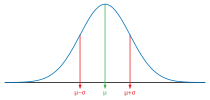
\includegraphics{Images/NormalDist.png}

\end{center}

\section{Chi Squared Variables} 

if $X_1,.....X_k$ are independent standard normal variables, then the sum of their squares 
\[
Q = \sum_{i=1}^k Z_i^2
\]
is distributed to the chi-squared distribution with k degrees of freedom. Written as:
\[
Q \sim \chi^2(k) \; or \; Q \sim \chi_k^2
\]

Used in hypothesis testing. Goodness of fit test, independence tests, and so on...


Notes $x'x$ is $\chi^2(n)$ distributed

\section{Cochran's Theorem} 
Cochran's theorem tells us about the distributions of partitioned sums of squares of normally distributed random variables. Under the assumption of normality, the various quadratic forms are independent and $\chi^2$ distributed.\\
\\
\bTheorem (Cochran's Theorem) 
Let $X_1, X_2,...,X_n $ be independent  $N(0,\sigma^2)$ distributed random variables and suppose that 
\[
\sum_{i=1}^n X_i^2 = Q_1 +Q_2+...+Q_k
\]
where $Q_1 +Q_2+...+Q_k$ are positive semi-definite quadratic forms in the random variables $X_1, X_2...,X_n, $that is ,

\[
Q_i = X^{'}A_i X \; i = 1,2,...,k
\]
We set the Rank of $A_i=r_i, \; i=1,2,...,k$ if 
\[
r_1+r_2+...+r_k =n
\]
Then we have that 
\begin{enumerate}
\item $Q_1 +Q_2+...+Q_k$ are independent
\item $Q_i \sim \sigma^2\chi^2(r_i)$
\end{enumerate}
\eTheorem
\textbf{Note} The rank of the matrix is the number of linearly independent rows/columns in the matrix $\equiv$ number of its non-zero eigenvalues.

\bLemma 
Let $x_q,x_2,...,x_n$ be real  numbers. Suppose that $\sum x_i^2$ can be split into a sum of positive semi-definite quadratic forms such as

\[
\sum_{i=1}^n x_i^2 = Q_1+Q_2+...+Q_k
\]
where $Q_i = x'A_ix$ and $rank Q_i =rank A_i = r_i, \; i = 1,2,..,k$. if $\sum r_i =n$ then there exist an orthogonal matrix C we can set x = Cy and we get:
\[
Q_1 = y_1^2+y_2^2+..+y_{r_1}^2
\]
\[
Q_2 =y_{r_1+1}^2+y_{r_1+2}^2+..+y_{r_1+r_2}^2
\]
\[
Q_3 = y_{r_1+r_2+1}^2+y_{r_1+r_2+2}^2+..+y_{r_1+r_2+r_3}^2
\]
\begin{center}
.\\
.\\
.\\
\end{center}
\[
Q_k = y_{n-r_k+1}^2 + y_{n-r_k+2}^2+..+y_n^2
\]

The different quadratic forms contain different y-variables and the number of terms in each $Q_i = r_i$ (the rank of $Q_i$). The $y_i^2$ end up in different sums, where we can use this fact to prove independence of the different quadratic forms. If $x_i^2$ can be split into a sum of positive semi-definite quadratic forms, then there is a projection orthogonal matrix $x=Cy$ or $C'x=y$ which means that each $y_i$ appears in only one resulting sum of squares. 
\eLemma

\Proof 
Let $X_1, X_2,...,X_n $ be independent  $N(0,\sigma^2)$ distributed random variables and suppose that 
\[
\sum_{i=1}^n X_i^2 = Q_1 +Q_2+...+Q_k
\]
where $Q_1 +Q_2+...+Q_k$ are positive semi-definite quadratic forms in the random variables $X_1, X_2...,X_n, $that is ,

\[
Q_i = X'A_iX, \; i = 1,2,...,k
\]
We set the Rank of $A_i=r_i, \; i=1,2,...,k$ if 
\[
r_1+r_2+...+r_k =n
\]
Then we have that 
\begin{enumerate}
\item $Q_1 +Q_2+...+Q_k$ are independent
\item $Q_i \sim \sigma^2\chi^2(r_i)$
\end{enumerate}
From lemma 1, we know that there exists a projection orthogonal matrix C such that the transformation X=CY yields
\[
Q_1 = Y_1^2+Y_2^2+..+Y_{r_1}^2
\]
\[
Q_2 =Y_{r_1+1}^2+Y_{r_1+2}^2+..+Y_{r_1+r_2}^2
\]
\[
Q_3 = Y_{r_1+r_2+1}^2+Y_{r_1+r_2+2}^2+..+Y_{r_1+r_2+r_3}^2
\]
\begin{center}
.\\.\\.\\
\end{center}
\[
Q_k = Y_{n-r_k+1}^2 + Y_{n-r_k+2}^2+..+Y_n^2
\]

We know that $Y^2$ occurs in exactly one $Q_j$ and the $Y_i$'s are all independent $N(0,\sigma^2)$ random variables because C is a projection orthogonal matrix, Cochran's theorem follows.


\section{Single Variable Regression Hypothesis Testing}
\[
H_0: \qquad y_i =\epsilon_i \qquad N(0,\sigma^2) \textrm{ where $\epsilon_i$ is a random variable}
\]
\[
H_a: \qquad y_i =\hat{\beta}x_i \hat{\epsilon_i} \textrm{( There is linear dependence)}
\]

from Least squares, we know that 
\[
\hat{\beta}_1 = (XX^T)^{-1}X^TY 
\]
\[
\hat{\beta}_1 = \frac{\sum_{i=1}^n x_i y_i}{\sum x_i^2} =\sum \alpha_i y_i
\]
A  linear combination of  $y_i$

Under the Null Hypothesis $H_0$
$y_i \textrm{ is a random variable}$ 
 and $y_i = \epsilon_i \textrm{ where }y\sim N(0,\sigma^2)$ and $\hat{\beta_i}\sim N(0,\frac{\sigma^2}{\sum x_i^2})$
 Thus the variance is
\[var(\sum \alpha_iy_i) = (\sum \alpha_i^2) var(y_i)\]
\[=(\sum \alpha^2) \sigma^2\ = \frac{\sum x_i^2 \sigma^2}{\sum(x_j^2)^2} \]
\[=\frac{\sigma^2}{\sum x_j^2}\]

then we have the distribution of the weight vector $\beta_1$ as 
\[ \beta_1 \sim N(0,\frac{\sigma^2}{\sum x_j^2}) \]

What is the probability of having a $\beta$ such that $Pr(\beta >\hat{\beta}|H_0)$ 

\begin{center}
    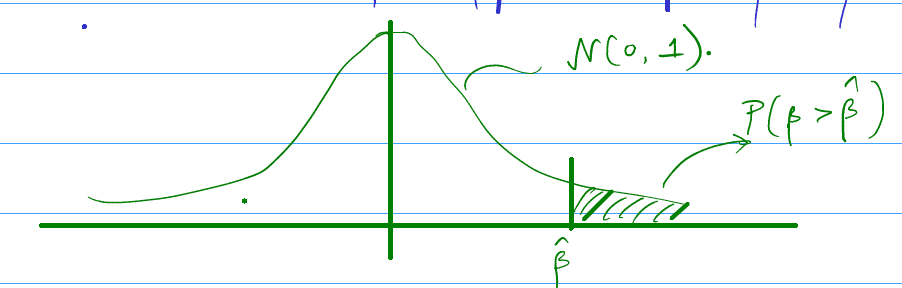
\includegraphics{Images/BetaProb.png}
\end{center}
for a value of $\sigma^2= \frac{y_i^2}{n}$ w/ mean of 0, otherwise $\sigma = \frac{(y_i - \Bar{Y}^2)}{n-1}$. We then have $\frac{\hat{\beta_1 -\mu}}{\hat{\sigma}}\to$ w/ mean 0 $\frac{\hat{\beta_1}}{\hat{\sigma}}$ \\

Since $\hat{\beta_1}$ and $\hat{\sigma^2}$ are complicated correlated, its hard to analyze the distribution of $\frac{\hat{\beta_1}}{\hat{\sigma^2}}$ . have the following defined by the Pythagorean theorem of the projection image below: 
\[
||y||^2 = (\hat{\beta_1}x)^2 + ||\epsilon_i||^2 = \sum y_i^2 = \hat{\beta_1}^2\sum x_i^2 + \sum \epsilon_i^2
\]
\begin{center}
    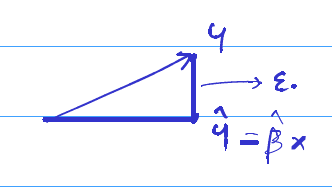
\includegraphics{Images/yHATProjection.png}
\end{center}

We divide through by  the variance $\sigma^2$ to get 
\[
\frac{\sum y_i^2}{\sigma^2} = \frac{\hat{\beta_1}^2\sum x_i^2}{\sigma^2} + \frac{\sum \epsilon_i^2}{\sigma^2}
\]
we then allow $u_i = \frac{ y_i}{\sigma_i}$ where $u_i \sim N(0,1)$, then
\[\sum_{i=1}^n u_i^2\sim \chi^2(n) \to \textrm{ (n degrees of freedom) and if }\]

\[ E[u_i^2]=1, \textrm{ then the mean is } n\]

Here we have 
\[
\frac{\sum y_i^2}{\sigma^2} = \frac{\hat{\beta_1}^2\sum x_i^2}{\sigma^2} + \frac{\sum \epsilon_i^2}{\sigma^2}
\]
and by Cochran's theorem, the two Right Hand Side factors are independent $\chi^2(1)$ and $ \chi^2(n-1)$ respectively. 
We note that $E[\frac{\sum \hat{\epsilon_i^2}}{\sigma^2}]= n-1$, and that $\hat{\sigma_2^2}= \frac{\sum \hat{\epsilon_i^2}}{n-1}  = \frac{\sum(y_i-\hat{\beta_1}x_i)^2}{n-1}$\\

We know that $\hat{\beta_1}$ is normally distributed and $\sigma_2^2$ is $\chi^2$ distributed with degrees of freedom $n-1$ and that the are independent. Thus, $\frac{\hat{\beta_1}}{\hat{\sigma_2}}\sim t(n-1)$, where $t(n-1)$ is the t-distribution with n-1 degrees of freedom.\\
The probability linear coefficient $\beta > \hat{\beta}(calculated)$ purely be chance is equivalent to the probability that a 
\[
t-statistic(n-2) > \frac{\hat{\beta }\sum x_i^2}{\sum \epsilon_i^2 / (n-2)}
\]
if small, we reject the null hypothesis in task 6
\section{Multiple Variable Regression Hypothesis Testing}
Given P parameters then let
$$x=\begin{pmatrix}
\vdots&&\vdots\\
x^{(1)}&\cdots&x^{(p)}\\
\vdots&&\vdots
\end{pmatrix}\text{ and } y=\begin{pmatrix}
y_1\\
\vdots\\
y_n
\end{pmatrix},$$

We say $||y||^2 = ||\hat{y}||^2 + ||\hat{\epsilon}||^2$ still holds and we still have
\[ 
||\hat{y}||^2 = \sum\hat{y_i}^2 = \sum y_i^2 - \sum\epsilon_i^2 \sim \sigma^2 \chi^2(p)
\]
\[ 
||\epsilon||^2= \sum \epsilon_i^2 \sim \chi^2(n-p-1)
\]
then 
\[
\frac{(\sum y^2 - \sum \epsilon^2)/p}{(\sum \epsilon^2)/(n-p-1)} \sim F(p,n-p-1)
\]
The probability under the null hypothesis that the data is similar purely by chance that we can see is
\[
Pr(F(p,n-p-1)) > \frac{(\sum y^2 - \sum \epsilon^2)/p}{(\sum \epsilon^2)/(n-p-1)} 
\]

if small, the the null hypothesis may be wrong. At least on of the features is significant. TASK 7

\section{F Test 1} 
\begin{itemize}
    \item $H_0$: None of the p-variables are relevant
    \item $H_a$: at least 1 p-variable is relevant
\end{itemize}

\section{F Test 2 } 
\begin{itemize}
    \item $H_0$: $\beta_{q+1}=\beta_{q+2}= ...=\beta_{p}$=0 home of the variables 
    \item $H_a$: at least 1 variable $q+1 ...p$ are relevant $\equiv$ not all $\beta_k, \: k=1...n$ equal 0
\end{itemize}
Can use the defined test statistic

\[
F^* = MSR/MSE \sim \frac{\frac{\sigma^2\chi^2(p-1)}{p-1}}{\frac{\sigma^2\chi^2(n-p)}{n-p}}
\]

The decision rule to control the  Type 1 error at $\alpha$ is
\[
if F^* \leq F(1-\alpha;p-1,n-p) \to H_0
\]
\[
if F^* > F(1-\alpha;p-1,n-p) \to H_a
\]
